\documentclass{article}
\usepackage[pdftex]{graphicx,color}
\usepackage{amsmath}
\usepackage{url}

\newcommand{\dealii}{{\textsc{deal.II}}}
\newcommand{\pfrst}{{\normalfont\textsc{p4est}}}
\newcommand{\trilinos}{{\textsc{Trilinos}}}
\newcommand{\aspect}{\textsc{Aspect}}

\begin{document}

\thispagestyle{empty}
\vspace*{.3\textheight}

\begin{centering}
  \parindent0pt
  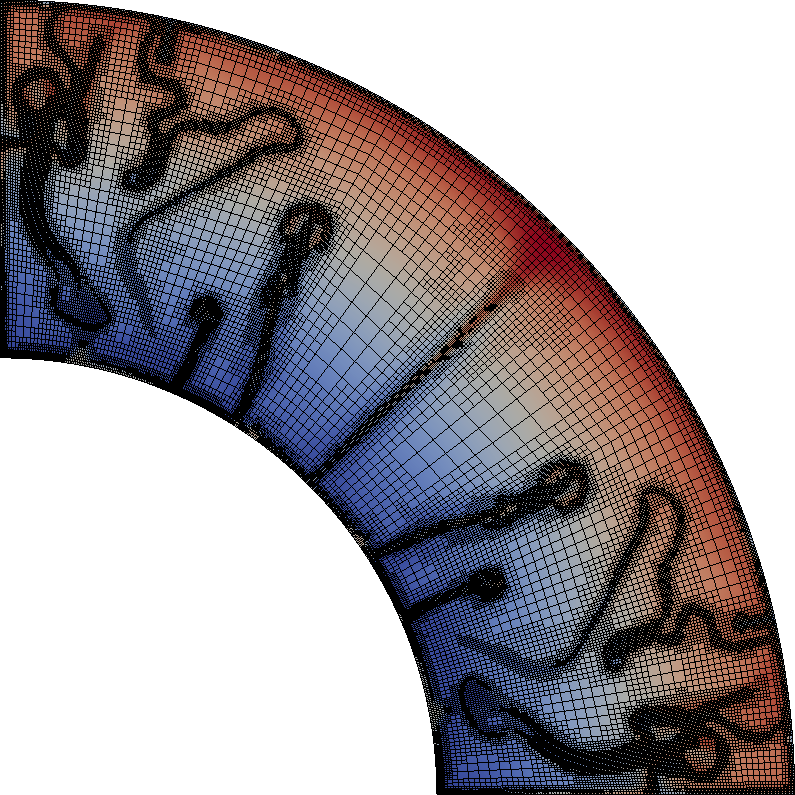
\includegraphics[width=0.6\textwidth]{mesh-2d.png}

  \vfill

  {\Large \aspect{} 0.8 preview release}
  \\[1cm]
  {\large
    Wolfgang Bangerth\\
    Timo Heister\\
    Martin Kronbichler\\
  }
\end{centering}


\pagebreak

\tableofcontents

\pagebreak

\section{Introduction}

\section{Equations, models, coefficients}

\subsection{Basic equations}

\aspect{} solves the following system of equations in a two- or
three-dimensional domain $\Omega$:
\begin{align}
  \label{eq:stokes-1}
  -\nabla \cdot 2\eta \varepsilon(\mathbf u) + \nabla p &=
  \rho \mathbf g
  & \qquad
  & \textrm{in $\Omega$},
  \\
  \label{eq:stokes-2}
  \nabla \cdot (\rho \mathbf u) &= 0
  & \qquad
  & \textrm{in $\Omega$},
  \\
  \label{eq:temperature}
  \rho C_p \left(\frac{\partial T}{\partial t} + \mathbf u\cdot\nabla T\right)
  - \nabla\cdot k\nabla T
  &=
  \rho\gamma
  +
  2\eta \varepsilon(\mathbf u) : \varepsilon(\mathbf u)
  +
  C_p T \frac{D\rho}{Dt}?
  \ or \ \rho C_p \frac{\partial\rho}{\partial p} \mathbf u\cdot\mathbf g
  ...
  & \qquad
  & \textrm{in $\Omega$},
\end{align}
where $\varepsilon(\mathbf u) = \frac{1}{2}(\nabla \mathbf u + \nabla\mathbf
u^T)$ is the symmetric gradient of the velocity (often called the
\textit{strain rate}).

In this set of equations, \eqref{eq:stokes-1} and \eqref{eq:stokes-2}
represent the compressible Stokes equations in which $\mathbf u=\mathbf
u(\mathbf x,t)$ is the velocity field and $p=p(\mathbf x,t)$ the pressure
field. Both fields depend on space $\mathbf x$ and time $t$. Fluid flow is
driven by the gravity force that acts on the fluid and that is proportional to
both the density of the fluid and the strength of the gravitational pull.

Coupled to this Stokes system is equation \eqref{eq:temperature} for the
temperature field $T=T(\mathbf x,t)$ that contains heat conduction terms as
well as advection with the flow velocity $\mathbf u$.
.......talk about rhs

These equations are
augmented by boundary conditions that can either be of Dirichlet-, Neumann, or
tangential type on subsets of the boundary $\Gamma=\partial\Omega$:
\begin{align}
  \mathbf u &= 0 & \qquad &\textrm{on $\Gamma_{0,\mathbf u}$},
  \\
  \mathbf n \cdot \mathbf u &= 0 & \qquad &\textrm{on $\Gamma_{\parallel,\mathbf u}$},
  \\
  T &= T_{\text{prescribed}}
   & \qquad &\textrm{on $\Gamma_{D,T}$},
  \\
  \mathbf n \cdot k\nabla T &= 0
   & \qquad &\textrm{on $\Gamma_{N,T}$}.
\end{align}
Here,
$\Gamma_{0,\mathbf u}$ corresponds to parts of the boundary on which the
velocity is fixed to be zero,
$\Gamma_{\parallel,\mathbf u}$ to parts of the boundary on which the
velocity may be nonzero but must be parallel to the boundary,
where
$\Gamma_{D,T}$ to places where the temperature is prescribed (for example at
the inner and outer boundaries of the earth mantle), and finally
$\Gamma_{N,T}$ to places where the temperature is unknown but the heat flux
across the boundary is zero (for example on symmetry surfaces if only a part
of the shell that constitutes the domain the Earth mantle occupies is
simulated). We require that one of these boundary conditions hold at each
point for both velocity and temperature, i.e.,
$\Gamma_{0,\mathbf u}\cup\Gamma_{\parallel,\mathbf u}=\Gamma$ and
$\Gamma_{D,T}\cup\Gamma_{N,T}=\Gamma$.

\aspect{} solves these equations in essentially the form stated. In
particular, the form given in \eqref{eq:stokes-1} implies that the pressure
$p$ we compute is in fact the \textit{total pressure}, i.e., the sum of
hydrostatic pressure and dynamic pressure.%
\footnote{Other codes often replace this equation by $-\nabla \cdot 2\eta
  \nabla \mathbf u + \nabla p_d =
  (\rho-\rho_0) \mathbf g$ where $p_d=(p+\rho_0 \varphi)$, and $\phi$ is the
  gravitational potential so that
  $\mathbf g=-\nabla\varphi$ and chosen in such a way that $\varphi=0$ at that
  part of the boundary where we want the pressure to be zero (e.g., on the
  earth surface). Furthermore, $\rho_0$ is a reference density. In this
  formulation, it is clear that the quantity that drives the fluid flow is in
  fact the \textit{buoyancy} caused by the \textit{variation} of densities,
  not the density itself. $p_d=p+\rho_0 \varphi$ is then the \textit{dynamic}
  pressure, i.e., the difference between total pressure and hydrostatic
  pressure $p_s=-\rho_0\varphi$.

  While this formulation has a number of numerical advantages, it also has
  significant disadvantages: (i) The pressure we compute is not immediately
  comparable to quantities that we need to look up pressure-dependent
  quantities such as the density. (ii) The definition of a reference density
  is only simple if we have incompressible models for which the density only
  depends on the temperature; for more complicated models, it is not a priori
  clear which density $\rho_0$ to chose so that $p+\rho_0 \varphi$ really only
  contains the dynamic part of the pressure. (iii) To compute the total
  pressure $p$ from $p_d$ one needs to know a gravitational potential
  $\varphi$ that is consistent with the gravity vector $\mathbf g$. This is
  not always trivial because many simple models just prescribe a $\mathbf g$
  for which no such potential needs to exist; for example, this is the case
  when using a radially inward gravitational vector of constant magnitude.}
Consequently, it allows the direct use of this pressure when looking up
pressure dependent material parameters.

In the implementation of these equataions, \aspect{} uses the SI unit system
throughout (i.e., it expresses all quantities in meters, kilograms and
seconds). All material parameters, geometries, etc., must also be expressed in
these units. For convenience, some rate-type output quantities are provided in
units \textit{per year} instead of \textit{per second}; however, this
conversion happens at the time output is generated, and is not part of the
solution process.


\subsection{Coefficients}

The equations above contain a significant number of coefficients that we will
discuss in the following. In the most general form, many of these coefficients
depend nonlinearly on the solution variables pressure $p$, temperature $T$
and, in the case of the viscosity, on the strain rate $\varepsilon(\mathbf
u)$. Alternatively, they may be parameterized as a function of the spatial
variable $\mathbf x$. \aspect{} allows both kinds of parameterizations.

\textbf{Note: The next version of \aspect{} will actually iterate out
  nonlinearities in the material description. However, in the current version,
  we simply evaluate all nonlinear dependence of coefficients at the solution
  variables from the previous time step or a solution suitably extrapolated from
  the previous time steps.}

Note that below we will discuss examples of the dependence of coefficients on
other quantities; which dependence is actually implemented in the code is a
different matter. As we will discuss in Section~\ref{sec:parameters} and
\ref{sec:extending}, some versions of these models are already implemented and
can be selected from the input parameter file; others are easy to add to
\aspect{} by providing self-contained descriptions of a set of coefficients
that the rest of the code can then use without a need for further
modifications.

Concretely, we consider the following coefficients and dependencies:
\begin{itemize}
\item \textit{The viscosity $\eta=\eta(p,T,\varepsilon(\mathbf u),\mathbf
    x)$:} Units $\textrm{Pa}\cdot \textrm{s} =
  \textrm{kg}\frac{1}{\textrm{m}\cdot\textrm{s}}$.

  The viscosity is the proportionality factor that relates total forces
  (external gravity minus pressure gradients) and fluid velocities $\mathbf
  u$. The simplest models assume that $\eta$ is constant, with the constant
  often chosen to be on the order of $10^{21} \textrm{Pa}\;\textrm{s}$.

  More complex (and more realistic) models assume that the viscosity depends
  on pressure, temperature and strain rate. Since this dependence is often
  difficult to quantify, one modeling approach is to make $\eta$ spatially
  dependent.

\item \textit{The density $\rho=\rho(p,T,\mathbf x)$:} Units
  $\frac{\textrm{kg}}{\textrm{m}^3}$.

  In general, the density depends on pressure and temperature, both through
  pressure compression, thermal expansion, and phase changes the material may
  undergo as it moves through the pressure-temperature phase diagram.

  The simplest parameterization for the density is to assume a linear
  dependence on temperature, yielding the form
  $\rho(T)=\rho_{\text{ref}}[1-\beta (T-T_{\text{ref}})]$ where
  $\rho_{\text{ref}}$ is the reference density at temperature $T_{\text{ref}}$
  and $\beta$ is the linear thermal expansion coefficient. For the earth
  mantle, typical values for this parameterization would be
  $\rho_{\text{ref}}=3300\frac{\textrm{kg}}{\textrm{m}^3}$,
  $T_{\text{ref}}=293 \textrm{K}$, $\beta=2\cdot 10^{-5}
  \frac{1}{\mathrm{K}}$.

\item \textit{The gravity vector $\mathbf g=\mathbf g(\mathbf x)$:} Units
  $\frac{\textrm{m}}{\textrm{s}^2}$.

  Simple models assume a radially inward gravity vector of constant magnitude
  (e.g., the surface gravity of Earth, $9.81 \frac{\textrm{m}}{\textrm{s}^2}$),
  or one that can be computed analytically assuming a homogenous mantle
  density.

  A physically self-consistent model would compute the gravity vector as
  $\mathbf g = -\nabla \varphi$ with a gravity potential $\varphi$ that
  satisfies $-\Delta\varphi=4\pi G\rho$ with the density $\rho$ from above and
  $G$ the universal constant of gravity. This would provide a gravity vector
  that changes as a function of time. Such a model is not currently
  implemented.

\item \textit{The specific heat capacity $C_p=C_p(p,T,\mathbf x)$:} Units
  $\frac{\textrm{J}}{\textrm{kg}\cdot\textrm{K}} =
  \frac{\textrm{m}^2}{\textrm{s}^2\cdot\textrm{K}}$.

  The specific heat capacity denotes the amount of energy needed to increase
  the temperature of one kilogram of material by one degree. Wikipedia lists a
  value of 790 $\frac{\textrm{J}}{\textrm{kg}\cdot\textrm{K}}$ for granite%
  \footnote{See \url{http://en.wikipedia.org/wiki/Specific_heat}.}
  For the earth mantle, a value of 1250
  $\frac{\textrm{J}}{\textrm{kg}\cdot\textrm{K}}$ is within the range
  suggested by the literature.


\item \textit{The thermal conductivity $k=k(p,T,\mathbf x)$:} Units
  $\frac{\textrm{W}}{\textrm{m}\cdot\textrm{K}}=\frac{\textrm{kg}\cdot\textrm{m}}{\textrm{s}^3\cdot\textrm{K}}$.

  The thermal conductivity denotes the amount of thermal energy flowing
  through a unit area for a given temperature gradient. It depends on the
  material and as such will from a physical perspective depend on pressure and
  temperature due to phase changes of the material as well as through
  different mechanisms for heat transport (see, for example, the partial
  transparency of perovskite, the most abundant
  material in the earth mantle, at pressures above around 120 GPa
  \cite{BRVMFG04}).

  As a rule of thumb for its
  order of magnitude, wikipedia quotes values of
  $1.83$--$2.90\frac{\textrm{W}}{\textrm{m}\cdot\textrm{K}}$ for sandstone and
  $1.73$--$3.98\frac{\textrm{W}}{\textrm{m}\cdot\textrm{K}}$ for granite.%
  \footnote{See \url{http://en.wikipedia.org/wiki/Thermal_conductivity} and
    \url{http://en.wikipedia.org/wiki/List_of_thermal_conductivities}.} The
  values in the mantle are almost certainly higher than this though probably
  not by much. The exact exact value
  is not really all that important: heat transport through convection is
  several orders of magnitude more important than through thermal
  conduction.

\item \textit{The intrinsic specific heat production $\gamma=\gamma(\mathbf x)$:} Units
  $\frac{\textrm{W}}{\textrm{kg}}=\frac{\textrm{m}^2}{\textrm{s}^3}$.

  This term denotes the intrinsic heating of the material, for example due to
  the decay of radioactive material. As such, it depends not on pressure or
  temperature, but may depend on the location due to different chemical
  composition of material in the earth mantle. The literature suggests a value
  of $\gamma=7.4\cdot 10^{-12}\frac{\textrm{W}}{\textrm{kg}}$.
\end{itemize}


\subsection{Numerical methods}

There is no shortage in the literature for methods to solve the equations
outlined above. The methods used by \aspect{} use the following,
interconnected set of strategies in the implementation of numerical
algorithms:
\begin{itemize}
\item \textit{Mesh adaptation:} Mantle convection problems are characterized
  by widely disparate length scales (from plate boundaries on the order of
  kilometers or even smaller, to the scale of the entire earth). Uniform
  meshes can not resolve the smallest length scale without an intractable
  number of unknowns.  Fully adaptive meshes allow resolving local features of
  the flow field without the need to refine the mesh globally. Since the
  location of plumes that require high resolution change and move with time,
  meshes also need to be adapted every few time steps.
\item \textit{Accurate discretizations:} The Boussinesq problem upon which
  most models for the earth mantle are based
  has a number of intricacies that make the choice of discretization
  non-trivial. In particular, the finite elements chosen for velocity and
  pressure need to satisfy the usual compatibility condition for saddle point
  problems. This can be worked around using pressure stabilization schemes for
  low-order discretizations, but high-order methods can yield better accuracy
  with fewer unknowns and offer more reliability. Equally important is the choice of
  a stabilization method for the highly advection-dominated temperature
  equation. \aspect{} uses a nonlinear artificial diffusion method for the latter.
\item \textit{Efficient linear solvers:} The major obstacle in solving the
  Boussinesq system is the saddle-point nature of the Stokes equations. Simple
  linear solvers and preconditioners can not efficiently solve this system in
  the presence of strong heterogeneities or when the size of the system
  becomes very large. \aspect{} uses an efficient solution strategy based on a
  block triangular preconditioner utilizing an algebraic multigrid that
  provides optimal complexity even up to problems with hundreds of millions of
  unknowns.
\item \textit{Parallelization of all of the steps above:} Global mantle convection
  problems frequently require extremely large numbers of unknowns for
  adequate resolution in three dimensional simulations. The only realistic way to solve such problems lies in
  parallelizing computations over hundreds or thousands of processors. This is
  made more complicated by the use of dynamically changing meshes, and it
  needs to take into account that we want to retain the optimal complexity of
  linear solvers and all other operations in the program.
\item \textit{Modularity of the code:} A code that implements all of these
  methods from \textit{scratch} will be unwieldy, unreadable and unusable as a community
  resource. To avoid this, we build our implementation on widely used and well
  tested libraries that can provide researchers interested in extending it
  with the support of a large user community. Specifically, we use the
  \dealii{} library \cite{BHK07,BK99m} for meshes, finite
  elements and everything discretization related; the \trilinos{} library
  \cite{trilinos,trilinos-web-page} for scalable and parallel linear algebra;
  and \pfrst{} \cite{p4est} for distributed, adaptive meshes. As a
  consequence, our code is freed of the mundane tasks of defining finite
  element shape functions or dealing with the data structures of linear algebra,
  can focus on the high-level description of what is supposed to happen, and
  remains relatively compact. The code will also
  automatically benefit from improvements to the underlying libraries with
  their much larger development communities. \aspect{} is extensively
  documented to enable other researchers to understand, test, use, and extend it.
\end{itemize}

Rather than detailing the various techniques upon which \aspect{} is built, we
refer to the paper by Kronbichler, Heister and Bangerth \cite{KHB12} that
gives a detailed description and rationale for the various building blocks.



\subsection{Variations on the basic equations}

Boussinesq approximation. Incompressible Stokes.

\section{Installation}

\section{Running \aspect}

Output in MKS, occasionally per year

\section{Input parameters}
\label{sec:parameters}

\section{Extending \aspect}
\label{sec:extending}

deal.II
documentation
dimension independent

plugins
existing plugins have header files so they show up in the documentation but
     this is not necessary

\bibliographystyle{unsrt}
\bibliography{manual}

\end{document}
